\documentclass[a4paper,12pt]{article}

% ---------- Encoding / Vietnamese ----------
\usepackage[utf8]{inputenc}
\usepackage[T5,T1]{fontenc}
\usepackage[vietnamese]{babel}

% ---------- Layout ----------
\usepackage[margin=2.5cm]{geometry}
\usepackage{graphicx}
\usepackage{booktabs}
\usepackage{longtable}
\usepackage{array}
\usepackage{xcolor}
\usepackage{hyperref}
\usepackage{float}
\usepackage{tikz}
\usetikzlibrary{shapes.geometric,arrows.meta,positioning,fit,calc}
\usepackage{fancyhdr}
\usepackage{titlesec}
\usepackage{enumitem}
\usepackage{caption}

\hypersetup{
    colorlinks=true,
    linkcolor=blue!50!black,
    urlcolor=blue!50!black,
    citecolor=blue!50!black,
    pdftitle={Bao cao ky thuat - He thong canh bao va cham JSN-SR04T va ESP-NOW},
    pdfauthor={ACLAB}
}

\setlength{\headheight}{15pt}
\pagestyle{fancy}
\fancyhf{}
\fancyhead[L]{Hệ thống cảnh báo va chạm — JSN-SR04T \& ESP-NOW}
\fancyhead[R]{\thepage}
\renewcommand{\headrulewidth}{0.4pt}

\titleformat{\section}{\large\bfseries}{\thesection.}{0.5em}{}
\titleformat{\subsection}{\normalsize\bfseries}{\thesubsection.}{0.5em}{}

\newcommand{\code}[1]{\texttt{#1}}

\title{\textbf{Báo cáo Kỹ thuật\\[4pt]
\large Hệ thống Cảnh báo Va chạm bằng Cảm biến Siêu âm JSN-SR04T\\
truyền dữ liệu trực tiếp bằng ESP-NOW}}
\author{ACLAB}
\date{\today}

\begin{document}

\maketitle

\begin{abstract}
\noindent
Báo cáo này mô tả trạng thái hiện tại của hệ thống nhúng cảnh báo va chạm sử dụng cảm biến siêu âm chống nước JSN-SR04T, vi điều khiển ESP32-S3 và màn hình cảm ứng LVGL. Dữ liệu khoảng cách được truyền \textbf{trực tiếp giữa hai board bằng ESP-NOW} — liên kết Wi-Fi cục bộ không qua điểm truy cập, bộ định tuyến hay máy chủ đám mây — và ngưỡng cảnh báo được đánh giá cục bộ ngay trên thiết bị hiển thị. Nội dung tập trung vào phần cứng đang sử dụng, công cụ/framework và lý do lựa chọn, các API chính được gọi trong firmware, cũng như các chức năng đã hoàn thiện và hướng phát triển tiếp theo của hệ thống ở trạng thái hiện hành.

\vspace{4pt}
\noindent\textbf{Mã nguồn:} \url{https://github.com/YdtTran/supersonic-warning-system}
\end{abstract}

\tableofcontents
\newpage

% =====================================================================
\section{Giới thiệu và phạm vi hệ thống hiện tại}

Hệ thống phát hiện vật cản/xe cộ ở khoảng cách gần bằng cảm biến siêu âm, truyền khoảng cách đã lọc trực tiếp sang node màn hình bằng \textbf{ESP-NOW}, nơi ngưỡng cảnh báo được đánh giá cục bộ và hiển thị theo thời gian thực; còi cảnh báo được điều khiển ngay trên node cảm biến.

Ở trạng thái hiện tại, hệ thống đã lắp đặt và vận hành trên phần cứng thật với \textbf{đầy đủ 6 cảm biến siêu âm} bao quanh xe (trước, sau, và hai cảm biến mỗi bên hông phủ nửa trước/nửa sau) theo đúng sơ đồ điểm mù (\emph{no-zone}) của xe tải.

Phiên bản trước của hệ thống định tuyến dữ liệu qua nền tảng đám mây \textbf{CoreIoT (ThingsBoard)} bằng MQTT và xử lý ngưỡng bằng Rule-Chain. Kiến trúc này đã được thay thế bằng ESP-NOW nhằm loại bỏ phụ thuộc vào hạ tầng mạng và giảm độ trễ cảnh báo — một hệ thống an toàn gắn trên xe di chuyển không nên ngừng hoạt động khi mất sóng Wi-Fi hoặc Internet. Mã nguồn CoreIoT vẫn được giữ lại trong cây nguồn để có thể khôi phục, nhưng không nằm trên đường dữ liệu hiện hành (Mục~\ref{sec:cloud}).

% =====================================================================
\section{Kiến trúc hệ thống hiện hành}

Hình~\ref{fig:dataflow} mô tả luồng dữ liệu hiện hành của hệ thống: cảm biến siêu âm truyền tín hiệu Trig/Echo tới node cảm biến; node cảm biến lọc nhiễu rồi gửi khoảng cách đã lọc \textbf{trực tiếp} sang node màn hình bằng ESP-NOW; node màn hình tự đánh giá ngưỡng cảnh báo cục bộ và hiển thị. Toàn bộ đường dữ liệu nằm gọn giữa hai board, không có thành phần trung gian nào.

\begin{figure}[H]
\centering
\begin{tikzpicture}[
    node distance=1.1cm,
    box/.style={rectangle, rounded corners, draw=black!70, thick,
                 minimum width=6.6cm, minimum height=1cm,
                 align=center, fill=blue!6},
    lbl/.style={font=\footnotesize\itshape, align=center}
]
\node[box] (sensor) {Cảm biến siêu âm JSN-SR04T\\\footnotesize 6 cảm biến (trước, sau, 2 mỗi bên hông)};
\node[box, below=of sensor] (node1) {ESP32-S3 Sensor Node\\\footnotesize \href{https://github.com/YdtTran/supersonic-warning-system/tree/main/firmware/sensor-node}{\code{firmware/sensor-node}} — đo, lọc, còi báo cục bộ};
\node[box, below=1.6cm of node1] (node2) {ESP32-S3 Waveshare Screen Node\\\footnotesize \href{https://github.com/YdtTran/supersonic-warning-system/tree/main/firmware/waveshare-screen}{\code{firmware/waveshare-screen}} — đánh giá hazard cục bộ,\\\footnotesize dashboard LVGL 800x480};

\draw[-{Latex[length=2.5mm]}, thick] (sensor) -- node[lbl, right] {Trig/Echo GPIO} (node1);
\draw[-{Latex[length=2.5mm]}, thick] (node1) -- node[lbl, right] {ESP-NOW trực tiếp\\30 bytes/gói, 2\,Hz\\(không qua AP/cloud)} (node2);
\end{tikzpicture}
\caption{Luồng dữ liệu hiện hành của hệ thống.}
\label{fig:dataflow}
\end{figure}

% =====================================================================
\section{Phần cứng đang sử dụng}

\begin{table}[H]
\centering
\small
\begin{tabular}{@{}p{3.4cm}p{10.5cm}@{}}
\toprule
\textbf{Thành phần} & \textbf{Mô tả} \\
\midrule
Vi điều khiển & Board \textbf{Yolo:Uno}, dựa trên \textbf{ESP32-S3-WROOM-1} (Dual-Core 240MHz, Wi-Fi/BLE, PSRAM Octal). \\
Cảm biến khoảng cách & \textbf{JSN-SR04T V3} — cảm biến siêu âm chống nước, đầu dò tách rời board mạch, chạy ở Mode 0 (vi điều khiển phát xung Trig, đo độ rộng xung Echo qua GPIO). Sử dụng \textbf{6 cảm biến}. \\
Màn hình hiển thị & \textbf{Waveshare ESP32-S3 Touch LCD 7"} — panel RGB $800\times480$, cảm ứng dung kháng \textbf{GT911} (I2C 400kHz), IO-expander \textbf{CH422G} (I2C, địa chỉ \code{0x24}/\code{0x38}) điều khiển backlight, reset cảm ứng, CS thẻ SD và MUX CAN. \\
Cảnh báo cục bộ & Còi buzzer trên chân \textbf{GPIO11} của Sensor Node, phản hồi tức thời không phụ thuộc đường truyền. \\
Ràng buộc chân GPIO & Chip ESP32-S3 bản \emph{Embedded PSRAM 8MB} chiếm \textbf{GPIO47/48} làm xung nhịp vi sai cho PSRAM; các chân này không dùng được cho tín hiệu Trig/Echo (Mục~\ref{sec:future}). \\
\bottomrule
\end{tabular}
\caption{Danh mục phần cứng chính đang sử dụng.}
\end{table}

\begin{figure}[H]
\centering
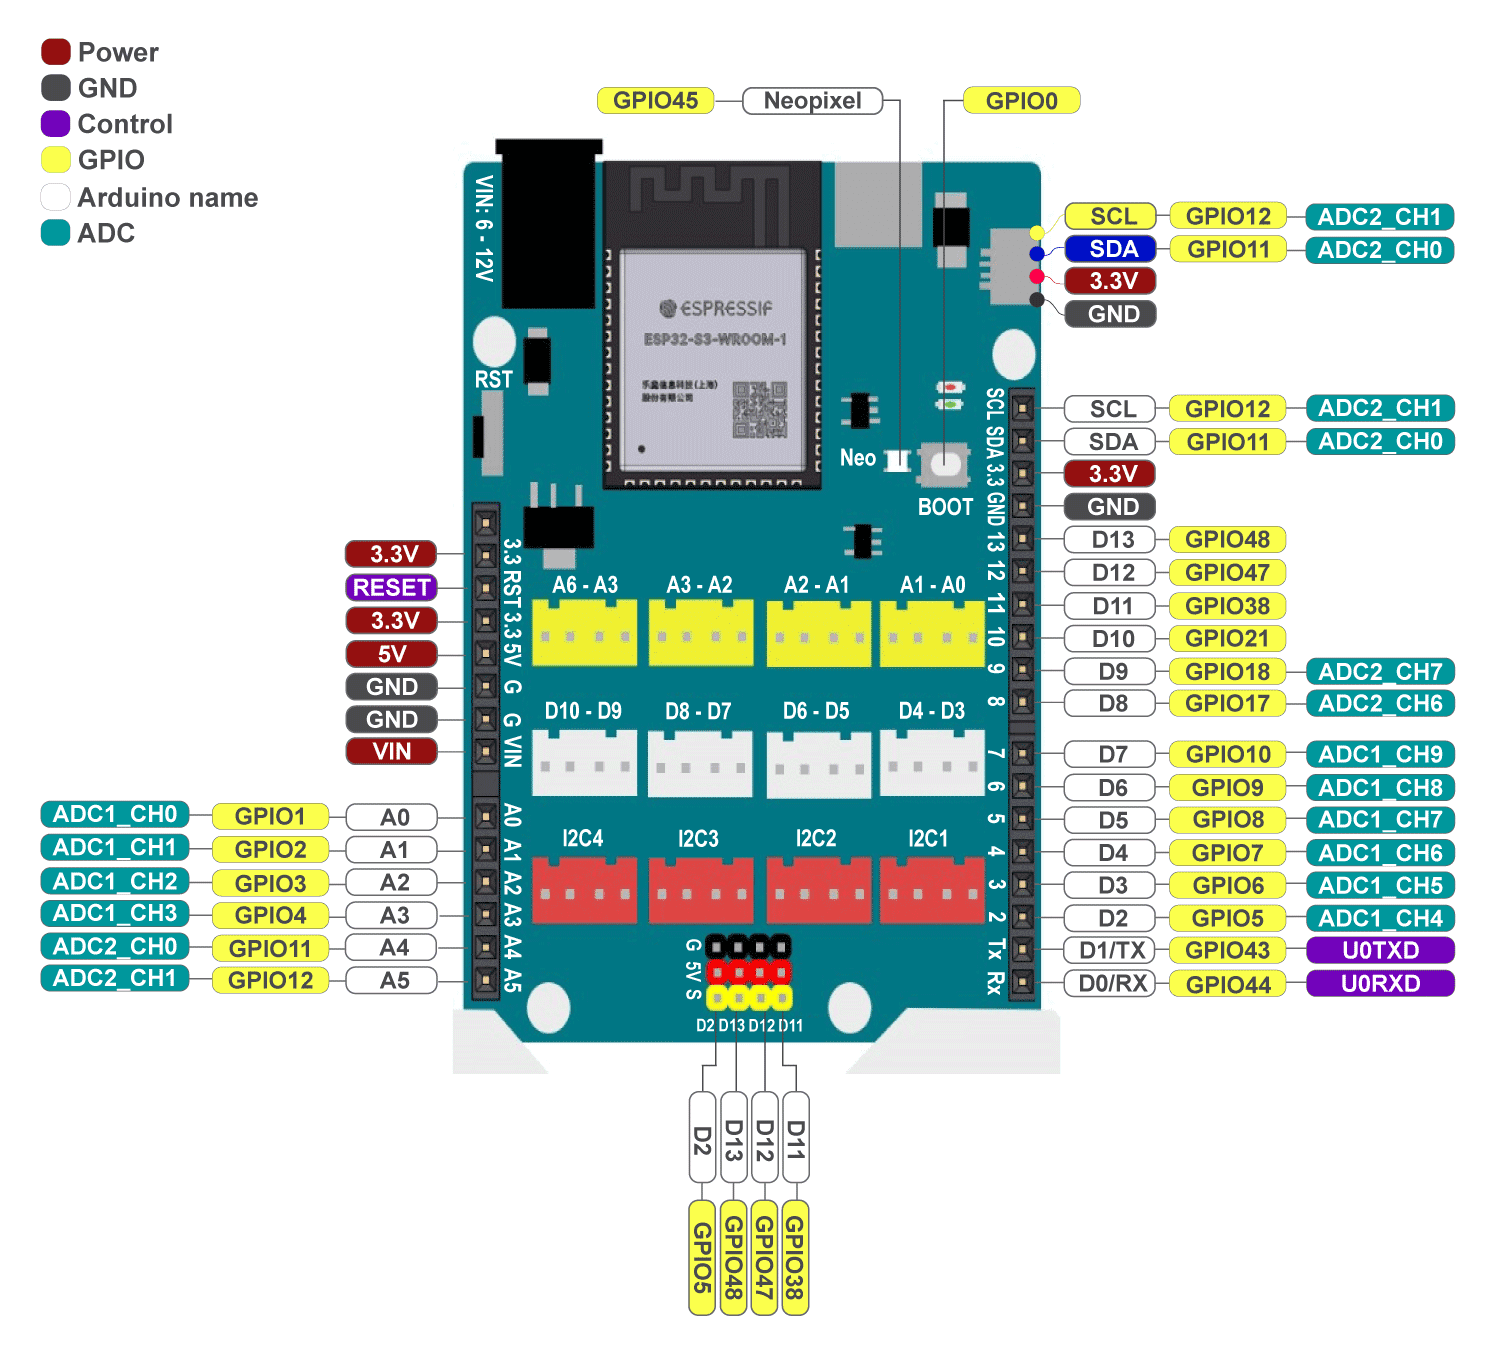
\includegraphics[width=0.92\textwidth]{image.png}
\caption{Sơ đồ pinout board Yolo:Uno (ESP32-S3).}
\end{figure}

\begin{figure}[H]
\centering
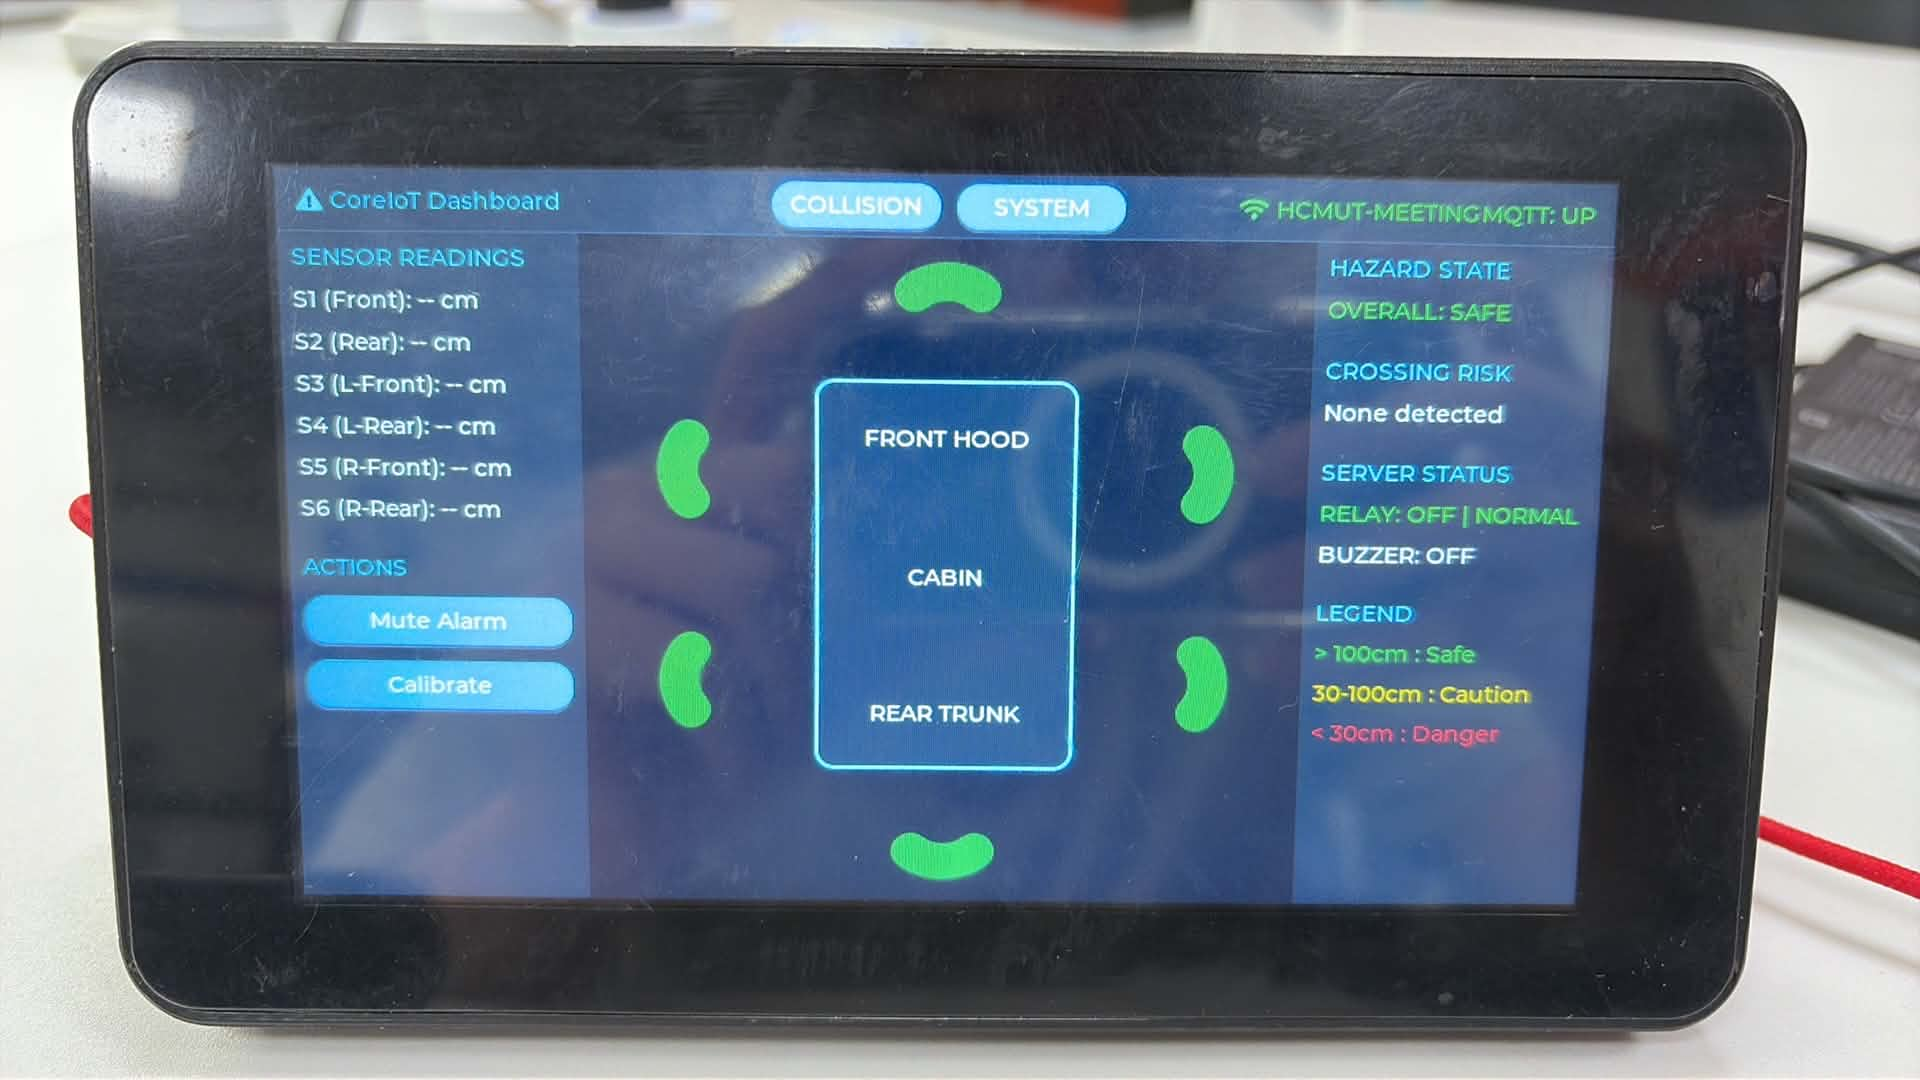
\includegraphics[width=0.72\textwidth]{dashboard-screen-img.jpg}
\caption{Dashboard cảnh báo va chạm chạy trên màn hình Waveshare LCD 7" (phần cứng thật).}
\end{figure}

% =====================================================================
\section{Công cụ và framework}

\begin{table}[H]
\centering
\small
\begin{tabular}{@{}p{3.0cm}p{4.4cm}p{6.5cm}@{}}
\toprule
\textbf{Hạng mục} & \textbf{Lựa chọn} & \textbf{Lý do} \\
\midrule
Build system & PlatformIO (\code{pio run -e yolo\_uno}) & Layout thống nhất cho cả hai firmware, một toolchain quản lý hai dự án khác framework. \\
\code{sensor-node} & \code{framework = arduino} & Tái sử dụng hệ sinh thái thư viện Arduino-ESP32 (\code{WiFi.h}, \code{esp\_now.h}) — đủ cho tác vụ đo/lọc/gửi ESP-NOW. \\
\code{waveshare-screen} & \code{framework = espidf} thuần & Driver màn hình/cảm ứng hiện đại (\code{esp\_lvgl\_adapter}, \code{esp\_lcd\_touch\_gt911}, LVGL 9.1, \code{esp\_lcd\_panel\_rgb}) đòi hỏi ESP-IDF $\geq 5.5$. \\
Đồ hoạ UI & LVGL 9.1 + \code{esp\_lvgl\_adapter} & Thư viện GUI nhúng mã nguồn mở phổ biến cho ESP32, adapter chính thức của Espressif quản lý vòng lặp render và khoá luồng an toàn. \\
Liên kết hai board & \textbf{ESP-NOW} (giao thức lớp 2 trên nền Wi-Fi radio) & Không cần AP/router/broker: hệ thống hoạt động cả khi không có mạng, độ trễ mỗi gói dưới $\approx$10\,ms, phù hợp cảnh báo va chạm thời gian thực. \\
Nền tảng IoT \emph{(không còn dùng)} & CoreIoT (ThingsBoard) & MQTT-native, Rule-Chain kéo-thả xử lý ngưỡng không cần backend riêng. Đã thay bằng ESP-NOW kết hợp đánh giá hazard cục bộ. \\
\bottomrule
\end{tabular}
\caption{Công cụ, framework sử dụng và lý do lựa chọn.}
\end{table}

% =====================================================================
\section{Firmware Sensor Node}

\subsection{Kiến trúc tác vụ FreeRTOS}

Bảng~\ref{tab:tasks-sensor} liệt kê các tác vụ FreeRTOS đang chạy trên \code{sensor-node}.

\begin{table}[H]
\centering
\small
\begin{tabular}{@{}lccc p{5.4cm}@{}}
\toprule
\textbf{Task} & \textbf{Stack} & \textbf{Priority} & \textbf{Core} & \textbf{Vai trò} \\
\midrule
\code{SensorTask} & 4096 & 2 & 1 & Trigger + đọc tuần tự từng cảm biến, đưa qua bộ lọc, ghi kết quả vào \code{SharedState}. \\
\code{AppTask} & 2048 & 1 & 1 & Tiêu thụ dữ liệu đã lọc song song, độc lập chu kỳ đo. \\
\code{NetworkTask} & 4096 & 1 & 0 & Đóng gói \code{SharedState} và gửi ESP-NOW sang node màn hình mỗi 500\,ms, tách khỏi core~1 để không ảnh hưởng timing đo. \\
\code{BuzzerTask} & 2048 & 1 & 0 & Đọc khoảng cách gần nhất, điều khiển còi vật lý GPIO11 theo ngưỡng WARNING/DANGER. \\
\bottomrule
\end{tabular}
\caption{Tác vụ FreeRTOS trên \code{sensor-node}.}
\label{tab:tasks-sensor}
\end{table}

\subsection{Bộ lọc khoảng cách (phân cụm + trung bình trượt mũ)}

Bộ lọc kết hợp phân cụm mẫu đo (loại outlier) và làm mượt bằng EMA (\emph{Exponential Moving Average}) để giảm nhiễu vốn có của cảm biến siêu âm giá rẻ mà vẫn phản ứng nhanh với thay đổi khoảng cách thật. Bảng~\ref{tab:filter} tóm tắt các tham số chính.

\begin{table}[H]
\centering
\small
\begin{tabular}{@{}lp{9.6cm}@{}}
\toprule
\textbf{Tham số} & \textbf{Ý nghĩa} \\
\midrule
Kích thước lịch sử & 9 mẫu RAW gần nhất được lưu để phân cụm. \\
Cụm hợp lệ tối thiểu & 5/9 mẫu phải thuộc cùng một cụm mới được chấp nhận. \\
Dung sai cụm & Cơ bản 8\,cm, tăng theo tỉ lệ 8\% so với khoảng cách đo (nhiễu tỉ lệ thuận khoảng cách). \\
Hệ số làm mượt EMA & 0.30. \\
Xác nhận bước nhảy & Một thay đổi lớn (>30\,cm hoặc >25\%) phải lặp lại 3 lần liên tiếp mới được chấp nhận, tránh nhiễu tức thời. \\
Reset bộ lọc & Sau 15 lần đọc lỗi liên tiếp. \\
\bottomrule
\end{tabular}
\caption{Tham số chính của bộ lọc khoảng cách.}
\label{tab:filter}
\end{table}

\subsection{Truyền dữ liệu bằng ESP-NOW}
\label{sec:espnow}

Node cảm biến gửi trực tiếp tới địa chỉ MAC của node màn hình bằng \code{esp\_now\_send()} (mã nguồn: \href{https://github.com/YdtTran/supersonic-warning-system/blob/main/firmware/sensor-node/src/EspNowClient.cpp}{\code{EspNowClient.cpp}}). Các đặc điểm chính:

\begin{itemize}[nosep]
    \item \code{WiFi.mode(WIFI\_STA)} chỉ để kích hoạt radio Wi-Fi; \textbf{không} gọi \code{WiFi.begin()} — không kết nối điểm truy cập nào, không broker, không phụ thuộc hạ tầng mạng.
    \item Kênh Wi-Fi cố định (kênh 1), bắt buộc trùng nhau ở cả hai board; địa chỉ MAC đích khai báo trong \code{EspNowConfig.h}.
    \item Payload là cấu trúc nhị phân đóng gói chặt (\emph{packed}) gồm \code{float[6]} khoảng cách và \code{uint8\_t[6]} cờ hợp lệ, tổng \textbf{30 byte} — chỉ chiếm 12\% giới hạn 250 byte mỗi gói của ESP-NOW v1.0. Cờ hợp lệ bằng 0 biểu thị cảm biến đang mất tín hiệu, để node màn hình hiển thị trạng thái ``không có dữ liệu'' thay vì giữ lại giá trị cũ.
    \item Tần suất gửi 2\,Hz (500\,ms), tách biệt với chu kỳ đo/lọc cục bộ 10\,Hz (100\,ms): bộ lọc vẫn phản ứng nhanh cho cảnh báo, chỉ giảm tải đường truyền.
\end{itemize}

Vì hai dự án dùng hệ thống biên dịch khác nhau (PlatformIO/Arduino và ESP-IDF) và không dùng chung đường dẫn header, cấu trúc bản tin phải được khai báo \textbf{trùng khớp thủ công} ở cả hai phía; tài liệu \code{docs/architecture/ESPNOW\_NETWORK.md} đóng vai trò nguồn thông tin dùng chung duy nhất về địa chỉ MAC, kênh và lược đồ dữ liệu.

\subsection{Cảnh báo còi cục bộ}

Còi buzzer được điều khiển trực tiếp trên \code{sensor-node} theo hai mức ngưỡng. Sau khi bỏ đường cloud, ngưỡng chỉ còn tồn tại một nơi duy nhất trong mã nguồn firmware nên không còn nguy cơ trôi lệch giữa còi vật lý và hiển thị màn hình:

\begin{itemize}[nosep]
    \item \textbf{WARNING} (20\,--\,50\,cm): kêu 1 lần mỗi 3 giây.
    \item \textbf{DANGER} ($<$20\,cm): kêu 1 lần mỗi 1 giây.
\end{itemize}

\begin{figure}[H]
\centering
\begin{tikzpicture}[
    every node/.style={font=\small},
    axis/.style={-{Latex[length=2.5mm]}, thick}
]
\draw[axis] (0,0) -- (10.5,0) node[right] {khoảng cách (cm)};
\foreach \x/\lbl in {0/0, 2/20, 5/50, 10/100} {
    \draw (\x,0.08) -- (\x,-0.08) node[below] {\lbl};
}
\draw[fill=red!25] (0,0) rectangle (2,0.6) node[midway,above=0.15cm] {DANGER};
\draw[fill=orange!30] (2,0) rectangle (5,0.6) node[midway,above=0.15cm] {WARNING};
\draw[fill=green!25] (5,0) rectangle (10.5,0.6) node[midway,above=0.15cm] {SAFE};
\end{tikzpicture}
\caption{Thang ngưỡng cảnh báo SAFE / WARNING / DANGER của còi buzzer cục bộ trên node cảm biến.}
\end{figure}

% =====================================================================
\section{Firmware Waveshare Screen}

\subsection{Nhận dữ liệu ESP-NOW và đánh giá hazard cục bộ}

Vì không sử dụng Arduino core, phần mạng dùng trực tiếp API ESP-IDF: \code{esp\_wifi.h}, \code{esp\_event.h}, \code{esp\_netif.h}, \code{esp\_now.h} và \code{nvs\_flash.h}. Logic nhận ESP-NOW nằm ngay trong \code{src/main.c}, \textbf{không tách thành component riêng} — \code{esp\_now} vốn là API hệ thống của ESP-IDF, không cần lớp bọc.

Tác vụ mạng khởi tạo Wi-Fi ở chế độ STA ``trần'' (không kết nối điểm truy cập nào), cố định kênh, rồi đăng ký hàm gọi lại \code{esp\_now\_register\_recv\_cb()}. Với mỗi bản tin nhận được, từng vị trí cảm biến được cập nhật hoặc xoá tuỳ theo cờ hợp lệ, sau đó hàm đánh giá hazard \textbf{tự tính trạng thái cảnh báo tổng thể} từ sáu vị trí cảm biến — thay cho vai trò của Rule-Chain trên đám mây trước đây.

Do ESP-NOW không có cơ chế \emph{heartbeat} ở tầng giao thức, một bộ định thời (\code{esp\_timer}) chu kỳ 1\,giây theo dõi thời điểm nhận gói cuối cùng; nếu quá 1{,}5\,giây không nhận được bản tin nào, phù hiệu trạng thái trên giao diện chuyển sang ``NO LINK'' để người vận hành biết liên kết đã mất.

\subsection{Mô hình dữ liệu cảm biến}

Component \code{sensor\_model} lưu trạng thái 6 cảm biến (khoảng cách, góc lắp, cờ dữ liệu cũ), được bảo vệ bằng một mutex FreeRTOS dùng chung. Mỗi khoảng cách được phân loại thành ba vùng: \textbf{SAFE} ($>$100\,cm), \textbf{CAUTION} (30\,--\,100\,cm), \textbf{DANGER} ($<$30\,cm).

\subsection{Giao diện LVGL 9.1}

Giao diện sử dụng các widget LVGL: \code{lv\_arc} (biểu diễn vùng cảm biến quanh xe), \code{lv\_label}, \code{lv\_anim} (hiệu ứng cảnh báo), \code{lv\_timer} (làm mới thông tin hệ thống định kỳ) và bố cục flex. Vì các tác vụ mạng chạy trên luồng (task) khác với luồng render LVGL, mọi thao tác cập nhật giao diện từ tác vụ mạng đều được bảo vệ bằng cơ chế khoá \code{esp\_lv\_adapter\_lock()} với thời gian chờ giới hạn 100\,ms, đảm bảo một luồng bị treo không làm treo toàn hệ thống.

\subsection{Lớp hỗ trợ phần cứng màn hình (BSP)}

Panel RGB $800\times480$ (RGB565) được khởi tạo qua \code{esp\_lcd\_new\_rgb\_panel()}, framebuffer đặt trong PSRAM. Bus I2C dùng API \code{driver/i2c\_master.h}, dùng chung cho IO-expander CH422G (ghi thanh ghi trực tiếp, không có driver riêng) và cảm ứng GT911 (driver chính thức \code{esp\_lcd\_touch\_gt911}) — mã nguồn: \href{https://github.com/YdtTran/supersonic-warning-system/blob/main/firmware/waveshare-screen/src/bsp/waveshare_rgb_lcd_port.c}{\code{waveshare\_rgb\_lcd\_port.c}}.

\begin{figure}[H]
\centering
\begin{tikzpicture}[
    node distance=0.9cm and 1.4cm,
    comp/.style={rectangle, rounded corners, draw=black!70, thick,
                 minimum width=4.2cm, minimum height=1.1cm, align=center, fill=orange!8},
]
\node[comp] (sm) {\href{https://github.com/YdtTran/supersonic-warning-system/tree/main/firmware/waveshare-screen/components/sensor_model}{\code{sensor\_model}}\\\footnotesize dữ liệu 6 cảm biến + mutex};
\node[comp, right=of sm] (cc) {\code{on\_data\_recv()} trong \code{src/main.c}\\\footnotesize ESP-NOW + watchdog liên kết};
\node[comp, below=1.3cm of $(sm)!0.5!(cc)$] (ui) {\href{https://github.com/YdtTran/supersonic-warning-system/tree/main/firmware/waveshare-screen/components/ui_dashboard}{\code{ui\_dashboard}}\\\footnotesize LVGL 9.1 + esp\_lv\_adapter lock};
\node[comp, below=of ui, fill=blue!8] (bsp) {BSP\\\footnotesize RGB panel / GT911 / CH422G};

\draw[-{Latex[length=2.2mm]}, thick] (cc) -- (ui);
\draw[-{Latex[length=2.2mm]}, thick] (sm) -- (ui);
\draw[-{Latex[length=2.2mm]}, thick] (ui) -- (bsp);
\end{tikzpicture}
\caption{Sơ đồ khối phần mềm của \code{waveshare-screen}.}
\end{figure}

% =====================================================================
\section{Kiến trúc CoreIoT trước đây (không còn sử dụng)}
\label{sec:cloud}

\begin{sloppypar}
Mục này mô tả kiến trúc \textbf{trước khi chuyển sang ESP-NOW}, giữ lại làm bối cảnh thiết kế và tài liệu tham chiếu cho khả năng khôi phục đường MQTT song song về sau. Rule-Chain hiện \textbf{không nằm trên đường dữ liệu}.
\end{sloppypar}

\begin{figure}[H]
\centering
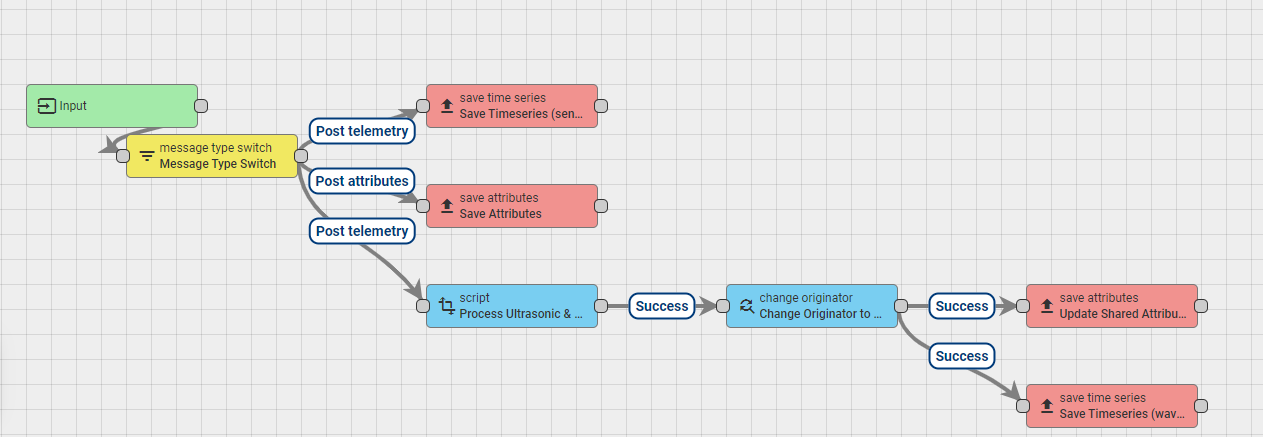
\includegraphics[width=0.95\textwidth]{rule-chain.png}
\caption{Rule-Chain CoreIoT của kiến trúc trước đây: xử lý dữ liệu telemetry và định tuyến sang node màn hình.}
\end{figure}

\begin{sloppypar}
Rule-Chain (\href{https://github.com/YdtTran/supersonic-warning-system/blob/main/cloud/coreiot/rule_chain/supersonic_rule_chain.json}{\code{supersonic\_rule\_chain.json}}) nhận bản tin telemetry từ \code{sensor-node}, script biến đổi (JavaScript) tính khoảng cách gần nhất trong các cảm biến, suy ra trạng thái \code{vehicle\_detected}, \code{warning\_status} (\code{NORMAL}/\code{WARNING}/\code{DANGER}) và \code{relay}; sau đó đổi chủ thể bản tin sang thiết bị \code{waveshare-screen} và đẩy dữ liệu xuống bằng cơ chế MQTT Shared Attributes (\code{notifyDevice=true}).
\end{sloppypar}

Lý do thay thế: ESP-NOW và Wi-Fi STA dùng chung radio, nên không thể vừa duy trì kết nối tới điểm truy cập vừa giữ liên kết ESP-NOW ổn định nếu hai bên khác kênh. Việc giữ song song hai đường truyền đòi hỏi đánh đổi độ ổn định, trong khi lợi ích của đường cloud (lưu lịch sử, giám sát từ xa) không thiết yếu với chức năng cảnh báo va chạm thời gian thực. Đổi lại, ngưỡng cảnh báo nay chỉ tồn tại trong firmware nên không còn nguy cơ trôi lệch giữa mã nguồn và cấu hình đám mây.

% =====================================================================
\section{Chức năng đã hoàn thiện}

\begin{itemize}[nosep]
    \item Đo và lọc khoảng cách ổn định từ \textbf{đầy đủ 6 cảm biến} siêu âm bao quanh xe.
    \item Truyền dữ liệu trực tiếp giữa hai board bằng ESP-NOW, hoạt động độc lập với hạ tầng mạng.
    \item Đánh giá ngưỡng cảnh báo \textbf{cục bộ ngay trên node màn hình}, không phụ thuộc xử lý phía đám mây.
    \item Phát hiện mất liên kết bằng bộ định thời giám sát, hiển thị rõ trạng thái ``NO LINK'' trên giao diện.
    \item Dashboard LVGL hiển thị trạng thái va chạm theo thời gian thực, kèm thông tin hệ thống (phiên bản firmware, bộ nhớ, thời gian hoạt động).
    \item Cảnh báo còi cục bộ trên \code{sensor-node}, phản hồi tức thời không phụ thuộc độ trễ mạng.
    \item Cơ chế khoá luồng an toàn giữa tác vụ mạng và tác vụ giao diện trên node màn hình.
\end{itemize}

% =====================================================================
\section{Hướng phát triển tiếp theo}
\label{sec:future}

\begin{itemize}[nosep]
    \item \textbf{Kiểm chứng tầm hoạt động ESP-NOW khi lắp cố định trên xe}: khoảng cách giữa hai board chỉ vài mét nên tầm xa không phải giới hạn, nhưng khung và động cơ kim loại có thể gây che chắn/nhiễu đáng kể — cần đo thực tế sau khi lắp đặt hoàn chỉnh.
    \item \textbf{Bật mã hoá cho liên kết ESP-NOW}: hiện đang truyền không mã hoá (\code{encrypt = false}). Chấp nhận được ở phạm vi cục bộ trong xe, nhưng nên bật CCMP (AES-128) nếu mở rộng phạm vi hoặc truyền thêm dữ liệu nhạy cảm.
    \item \textbf{Kênh điều khiển ngược từ màn hình về node cảm biến}: nút ``Mute Alarm'' hiện chỉ tắt cảnh báo hình ảnh trên màn hình, chưa tắt được còi vật lý — cần bổ sung liên kết ESP-NOW hai chiều.
    \item \textbf{Dọn hai dòng trạng thái tồn dư của kiến trúc MQTT trên giao diện}: dòng \code{BUZZER} và \code{RELAY} vốn hiển thị kết quả do Rule-Chain tính; sau khi bỏ đường đám mây, chúng không còn nguồn dữ liệu nên đứng yên vĩnh viễn. Cần xoá khỏi giao diện, hoặc bổ sung các trạng thái này vào bản tin ESP-NOW để hiển thị đúng.
    \item Bổ sung cảnh báo cho người đi đường phía ngoài xe (còi/đèn ngoài xe).
\end{itemize}

\end{document}
